%%%%%%%%%%%%%%%%%%%%%%%%%%%%%%%%%%%%%%%%%%%%%%%%%%%%%%%%%%%%%%%%%%%%%%%%%%%%
\chapter{Application: AM Radio}
In this chapter, we'll design a simple AM radio tuner circuit to tune into some AM radio station like AM 1010.

\begin{alevel}
What do AM and FM stand for?
\end{alevel}

When discussing radio stations, we often leave off the unit. AM 1010 means 1,010,000 Hz. We're looking to tune into electromagnetic waves at that frequency. These electromagnetic waves have an electric field component that causes electrons to slosh back and forth in the antenna. This causes a small voltage difference on the antenna which our circuit is trying to detect.

\begin{alevel}
What frequency is FM 98.1? What angular frequency corresponds to this?
\end{alevel}

We have lots of different types of electromagnetic waves, characterized by their frequency. 

\begin{blevel}
Fill in the Table~\ref{T:9L}. If the category is a range, present your answer accordinly.
\end{blevel}

\begin{table}[H]
\begin{center}
\begin{tabular}{c|c|c}
type of light&frequency&wavelength\\ \hline
red light&& \\ \hline
UV&& \\ \hline
AM radio&& \\ \hline
microwave oven&& \\ \hline
your cell phone&& \\ \hline
5G&& \\ \hline
An object at $300^0$C&& \\ \hline
\end{tabular}
\caption{Electromagnetic Spectrum Summary Table}
\label{T:9L}
\end{center}
\end{table}

When designing our radio tuner, we want a circuit that let's through frequencies close to 1010AM but blocks frequencies that are even a little bit larger or smaller. For example, we need to block AM 1020 and AM 1000. Let's define block as reducing its magnitude by a factor of 10.\par

One design idea is to use a voltage divider like the one shown here.

\begin{figure}[H]
\begin{center}
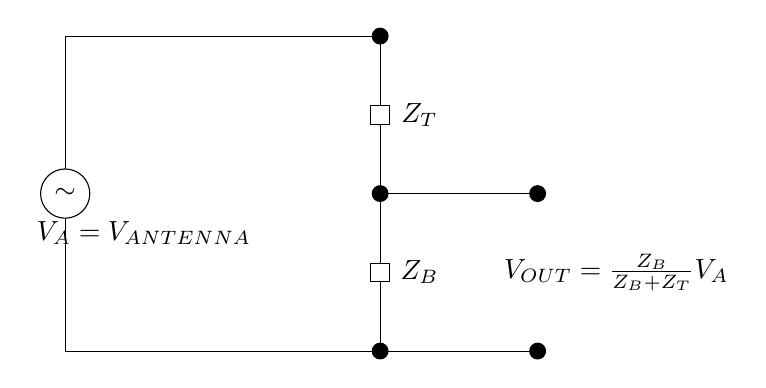
\begin{tikzpicture}
\draw (0,0)--(0,2) node[circle, draw=black, fill=white]{$\sim$}--(0,4)
--(4,4)--(4,3)node[draw=black, fill=white]{}
--(4,1)node[draw=black, fill=white]{}
--(4,0)--(0,0);
\filldraw (4,4) circle[radius=1 mm];
\filldraw (4,2) circle[radius=1 mm];
\filldraw (4,0) circle[radius=1 mm];
\draw node at (4.5,3) {$Z_T$};
\draw node at (4.5,1) {$Z_B$};
\draw node at (1,1.5) {$V_A=V_{ANTENNA}$};
\filldraw (6,2) circle[radius=1 mm];
\filldraw (6,0) circle[radius=1 mm];
\draw (4,2)--(6,2) (4,0)--(6,0);
\draw node at (7,1) {$V_{OUT}=\frac{Z_B}{Z_B+Z_T}V_A$};
\end{tikzpicture}
\caption{Radio tuner rough design idea}
\end{center}
\end{figure}

At a frequency of AM 1010, we want the ratio $r=\frac{Z_B}{Z_B+Z_T}$ to be very close to 1. At AM 1000 we want this ratio to be less than 0.1. \par

To get a ratio close to 1, we want $Z_B$ to be close to infinity. We have encounter this earlier, the parallel LC circuit has infinite impedance at resonance and finite impedance at other frequencies.\par

\begin{figure}[H]
\begin{center}
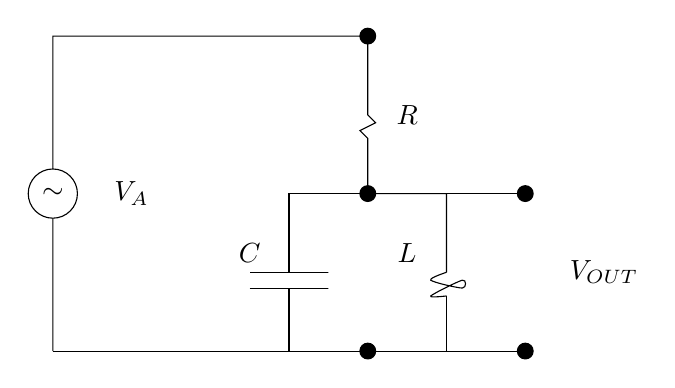
\begin{tikzpicture}
\draw (0,0)--(0,2) node[circle, draw=black, fill=white]{$\sim$}--(0,4)
--(4,4)--(4,3)--(4.1,2.9)--(3.9,2.8)--(4,2.7)--(4,2)--(5,2)--(5,1);
\draw (4,2)--(3,2)--(3,1)--(3.5,1)--(2.5,1) (2.5,.8)--(3.5,.8)--(3,.8)--(3,0);
\filldraw (4,4) circle[radius=1 mm];
\filldraw (4,2) circle[radius=1 mm];
\filldraw (4,0) circle[radius=1 mm];
\draw node at (4.5,3) {$R$};
\draw node at (2.5,1.25) {$C$};
\draw node at (4.5,1.25) {$L$};
\draw node at (1,2) {$V_A$};
\filldraw (6,2) circle[radius=1 mm];
\filldraw (6,0) circle[radius=1 mm];
\draw (4,2)--(6,2) (4,0)--(6,0);
\draw node at (7,1) {$V_{OUT}$};
\draw plot [smooth] coordinates {(5,1) (4.8,0.9) (5.2,.8) (5.2,.9) (4.8,.7) (5,.7)};
\draw (5,.7)--(5,0)--(4,0)--(0,0);
\end{tikzpicture}
\caption{Radio tuner with more details}
\end{center}
\end{figure}

Let's choose an inductance value of 30mH \footnote{Maybe we have one laying around.} and then solve for the needed value for the capacitance such that the resonance frequency is exactly 1010000 Hz ($\omega=2\pi 1010000 \frac{rad}{s}$).

\begin{align}
Z_B=Z_C \parallel Z_L \rightarrow Z_B=\frac{Li\omega\frac{1}{Ci\omega}}{Li\omega+\frac{1}{Ci\omega}} \notag \\
Z_B=\frac{\frac{L}{C}}{Li\omega-\frac{i}{C\omega}} \label{E:9ZB}
\end{align}

The denomonator is zero when $C=\frac{1}{L\omega^2}=0.8277063pF$.\footnote{We need to keep lots of significant figures because we are comparing to a similar frequency. An alternative, but slightly more sophisticated method is to......} This makes the ratio, r, equal to 1 at 1010AM because at this frequency the impedance $Z_B \rightarrow \infty$.\par

Next, we need to make sure that at AM 1020 and AM 1000, that our ratio, r, is 0.1 or less. We need to pick a value of R big enough to make this so. According to equation~\eqref{E:9ZB}, at AM 1010, $Z_B=i1.57E12\Omega$.

\begin{align}
r=0.1 = \frac{Z_B}{R+Z_B}=\frac{i1.57E12}{R+i1.57E12}\notag \\
R \approx 1.57E13 \Omega
\end{align}
 We have several practical problems, like the inductance has some resistance that we didn't account for and that our final resistor value is HUGE. If we actually want to listen to anything we need to send the output into some sort of amplifier. Op-amps have large input resistances, so large that we ignored them earlier in the book, but our R is so big that maybe we can't ignore that either.

\begin{clevel}
Draw the entire AM radio tuner/amplifier circuit. Include a non-inverting op-amp amplifier with a gain of 10.
\end{clevel}

\begin{clevel}
What value of capacitance would be needed to tune into AM 910?
\end{clevel}

\begin{clevel}
If this capacitor were made from two overlapping metal plates, spaced 1 mm apart what area of overlap would be needed for AM 910? What are of overlap would be needed for AM 1010?
\end{clevel}
